\documentclass{article}

\usepackage{graphicx}
\graphicspath{ {images} }
 
\usepackage{mathtools}

\usepackage{amsthm}
\renewcommand{\qedsymbol}{$\blacksquare$}
\usepackage{amssymb}
\usepackage{amsmath}
\newcommand\numberthis{\addtocounter{equation}{1}\tag{\theequation}}

\usepackage{hyperref}
\hypersetup{
    colorlinks = true,
}


\usepackage{titling}
\title{Exercise Set 2 - Reinforcement Learning}
\newcommand{\subtitle}[1]{%
  \posttitle{%
    \par\end{center}
    \begin{center}\large#1\end{center}
    \vskip0.5em}%
}
\makeatother
\subtitle{Tabular Methods}
\author{Giulio Starace - 13010840}
\date{\today}

\begin{document}
\maketitle
\section*{Homework: Coding Assignment - Monte Carlo}
\begin{enumerate}
	\item To derive the incremental update rule of the value function for a given state $V(s)$ using
	      ordinary importance sampling, we begin with the definition of the estimate $V_n(s)$ given $n$
	      sampled returns $G_1, \dots, G_n$ under this regime:
	      \begin{equation}\label{eq:value_function_estimate}
		      V_n(s) = \frac{1}{n} \sum^n_{k=1} W_k G_k,
	      \end{equation}
	      where $W_k$ is the importance sampling ratio of target policy $\pi$ over behavior policy $b$.
	      \begin{equation}
		      W_k = \rho_{t_k:T(t_k)-1} = \prod_{t=t_k}^{T(t_k)-1} \frac{\pi(A_t|S_t)}{b(A_t|S_t)}.
	      \end{equation}
	      We expand equation (\ref{eq:value_function_estimate}) to obtain:
	      \begin{align*}
		      V_n(s) & = \frac{1}{n} \left[W_{n-1} G_{n-1} \sum^{n-1}_{i=1}W_kG_k\right]                  \\
		             & = \frac{1}{n} \left[W_{n-1} G_{n-1}
		      (n-1)\underbracket{\left(\frac{1}{n-1}\right)\sum^{n-1}_{i=1}W_kG_k}\right]                 \\
		             & =  \frac{1}{n} \left[W_{n-1} G_{n-1}(n-1)\underbracket{V_{n-1}(s)} \right]         \\
		             & = \frac{1}{n} \left[W_{n-1} G_{n-1}+ n V_{n-1}(s) - V_{n-1}(s)\right]              \\
		      V_n(s) & =  V_{n-1}(s) + \frac{1}{n} \left[W_{n-1} G_{n-1} - V_{n-1}(s)\right]. \numberthis
		      \label{eq:incremental_update_rule}
	      \end{align*}
	      We see that equation (\ref{eq:incremental_update_rule}) is of the form
	      \begin{equation}
		      V_n = V_{n-1} + \alpha * \left(\beta - V_{n-1}\right),
	      \end{equation}
	      with $\alpha = \frac{1}{n}$ and $\beta = W_{n-1} G_{n-1}$.  \\ \qed

	\item Coding answers have been submitted on codegra under the group ``stalwart cocky sawly".
	      Please refer to Figures \ref{fig:figure_5.1} and \ref{fig:v_function} for the requested figures.
	      \begin{figure}
		      \centering
		      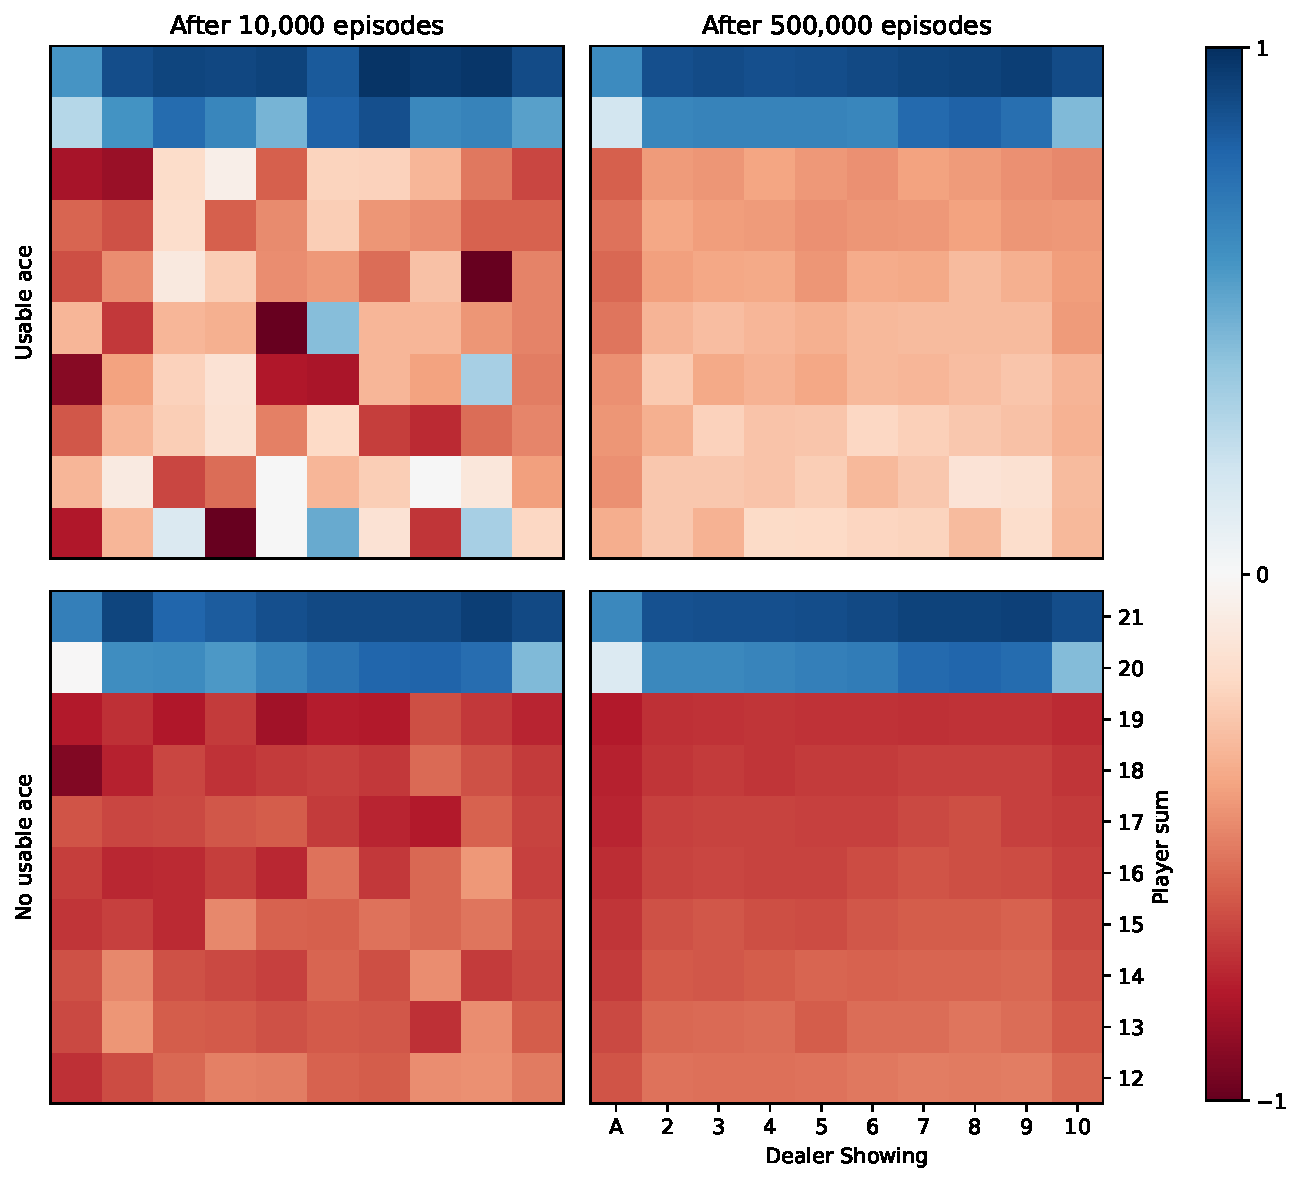
\includegraphics[width=\textwidth]{fig_5.1}
		      \caption{Blackjack value function across state configurations after 10k and 500k episodes.
			      Reproduction of figure 5.1 from Sutton and Barto, using heatmaps.}
		      \label{fig:figure_5.1}
	      \end{figure}
	\item let's go
\end{enumerate}

\section*{Homework: SARSA and Q-learning}
\begin{enumerate}
	\item \begin{enumerate}
		      \item hey
		      \item ho
	      \end{enumerate}
	\item \begin{enumerate}
		      \item hey
		      \item ho
	      \end{enumerate}
	\item let's go
\end{enumerate}


\end{document}
